% From runs to cell readings: an illustrative reading matrix.
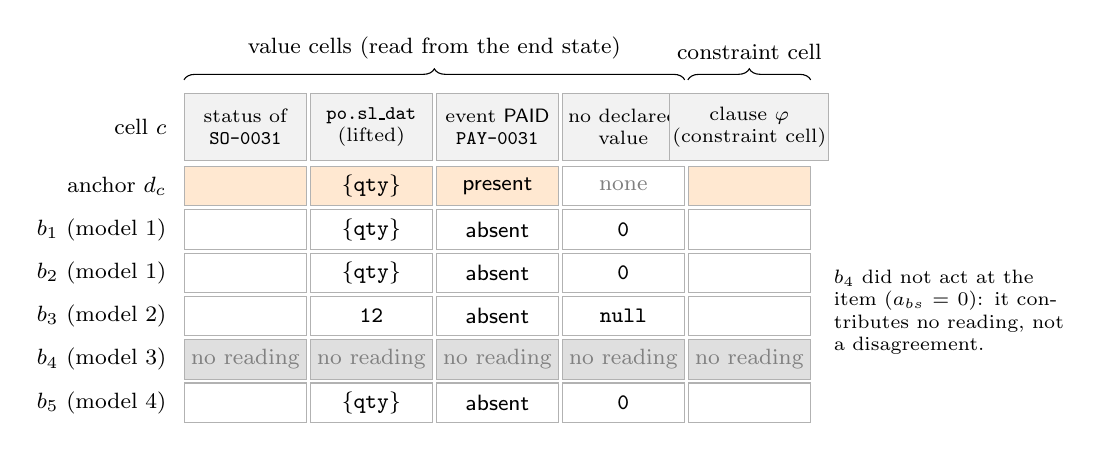
\begin{tikzpicture}[
  every node/.style={font=\footnotesize},
  cell/.style={draw=gray!60, minimum width=1.55cm, minimum height=0.5cm, inner sep=1pt},
  hd/.style={cell, fill=gray!10, font=\scriptsize, align=center, minimum height=0.85cm},
  an/.style={cell, fill=orange!18},
  miss/.style={cell, fill=gray!25, text=gray}]
\def\W{1.6}
% header
\node[anchor=east] at (-0.88,0.4) {cell $c$};
\foreach \i/\h in {0/{status of\\\texttt{SO-0031}}, 1/{\texttt{po.sl\_dat}\\(lifted)}, 2/{event \textsf{PAID}\\\texttt{PAY-0031}}, 3/{no declared\\value}, 4/{clause $\varphi$\\(constraint cell)}}
  \node[hd] at (\i*\W,0.4) {\h};
\node[anchor=east] at (-0.88,-0.35) {anchor $d_c$};
\foreach \i/\v in {0/{\viCho}, 1/{\texttt{\{qty\}}}, 2/{\textsf{present}}, 4/{\sat}}
  \node[an] at (\i*\W,-0.35) {\v};
\node[cell, fill=white, text=gray] at (3*\W,-0.35) {none};
% readings
\foreach \r/\lab/\va/\vb/\vc/\vd/\ve in {
  1/{$b_1$ (model 1)}/{\viDa}/{\texttt{\{qty\}}}/{\textsf{absent}}/{\texttt{0}}/{\sat},
  2/{$b_2$ (model 1)}/{\viCho}/{\texttt{\{qty\}}}/{\textsf{absent}}/{\texttt{0}}/{\viol},
  3/{$b_3$ (model 2)}/{\viDa}/{\texttt{12}}/{\textsf{absent}}/{\texttt{null}}/{\sat},
  4/{$b_4$ (model 3)}/{--}/{--}/{--}/{--}/{--},
  5/{$b_5$ (model 4)}/{\viDa}/{\texttt{\{qty\}}}/{\textsf{absent}}/{\texttt{0}}/{\sat}} {
  \node[anchor=east] at (-0.88,-0.35-0.55*\r) {\lab};
  \ifnum\r=4
    \foreach \i in {0,...,4} \node[miss] at (\i*\W,-0.35-0.55*\r) {no reading};
  \else
    \node[cell] at (0,-0.35-0.55*\r) {\va};
    \node[cell] at (\W,-0.35-0.55*\r) {\vb};
    \node[cell] at (2*\W,-0.35-0.55*\r) {\vc};
    \node[cell] at (3*\W,-0.35-0.55*\r) {\vd};
    \node[cell] at (4*\W,-0.35-0.55*\r) {\ve};
  \fi
}
% braces
\draw[decorate, decoration={brace, amplitude=4pt}] (-0.78,1.0) -- (3*\W+0.78,1.0) node[midway, above=4pt] {value cells (read from the end state)};
\draw[decorate, decoration={brace, amplitude=4pt}] (4*\W-0.78,1.0) -- (4*\W+0.78,1.0) node[midway, above=4pt, align=center] {constraint cell};
\node[anchor=west, align=left, font=\scriptsize, text width=3.0cm] at (4*\W+0.95,-1.95) {$b_4$ did not act at the item ($a_{bs}=0$): it contributes no reading, not a disagreement.};
\end{tikzpicture}
